\documentclass{beamer}	
\mode<presentation>
 
\usepackage{pdfpages}
\usepackage{fancyvrb}
\usepackage{chemarr}

\usepackage{amsmath}		%% mathematics typesetting
\usepackage{amssymb}
 
\usepackage{epigraph}   %% nice setting of quotations

\usepackage{tabularx} %% allows to use row colours in tables

\usepackage{ulem}

\usepackage{booktabs}

\usepackage{siunitx} %% tpyeset SI units

\usepackage{CJKutf8} %% typeset Chinese characters

\usepackage{pdfpages}%% include pdfs

\usepackage{graphicx}
\usepackage{animate} %% show animated gifs

\DeclareMathAlphabet{\mathcalligra}{T1}{calligra}{m}{n}


% Color and Theme. Can be changed. However, this one's quite nice.
\usetheme{Madrid}
\definecolor{theme}{rgb}{0.84,0,0.21}
\usecolortheme[named=theme]{structure}

%%  Title information
\title[M11.13.6 Visuelles System II]{M11.13.6 Visuelles System II: \\ Retinale Signalverarbeitung und zentrale Sehbahn}
\author[melanie.stefan@medicalschool-berlin.de]{}
\institute[]{Prof. Melanie Stefan \\ melanie.stefan@medcialschool-berlin.de}
\date{WiSe 2022/23}
 

% Table of contents to pop up at the beginning of each section
\AtBeginSection[]
{
  \begin{frame}<beamer>
    \frametitle{Outline}
    \tableofcontents[currentsection,currentsubsection]
  \end{frame}
}
 
\beamertemplatenavigationsymbolsempty

\begin{document}


{ \usebackgroundtemplate{
\includegraphics[width=1.2\paperwidth]{MSB_Titelseite.pdf}} 
\begin{frame}

 \maketitle 

$\,$\\[6cm] 


\end{frame} 
}


%% Hook:

%% Bild Myopia, erste Vorlesung, wie geht es jetzt weiter? 
\begin{frame}{Sie wissen jetzt viel über den optischen Apparat}

\begin{columns}[c]

\begin{column}{5cm}
\begin{center}
    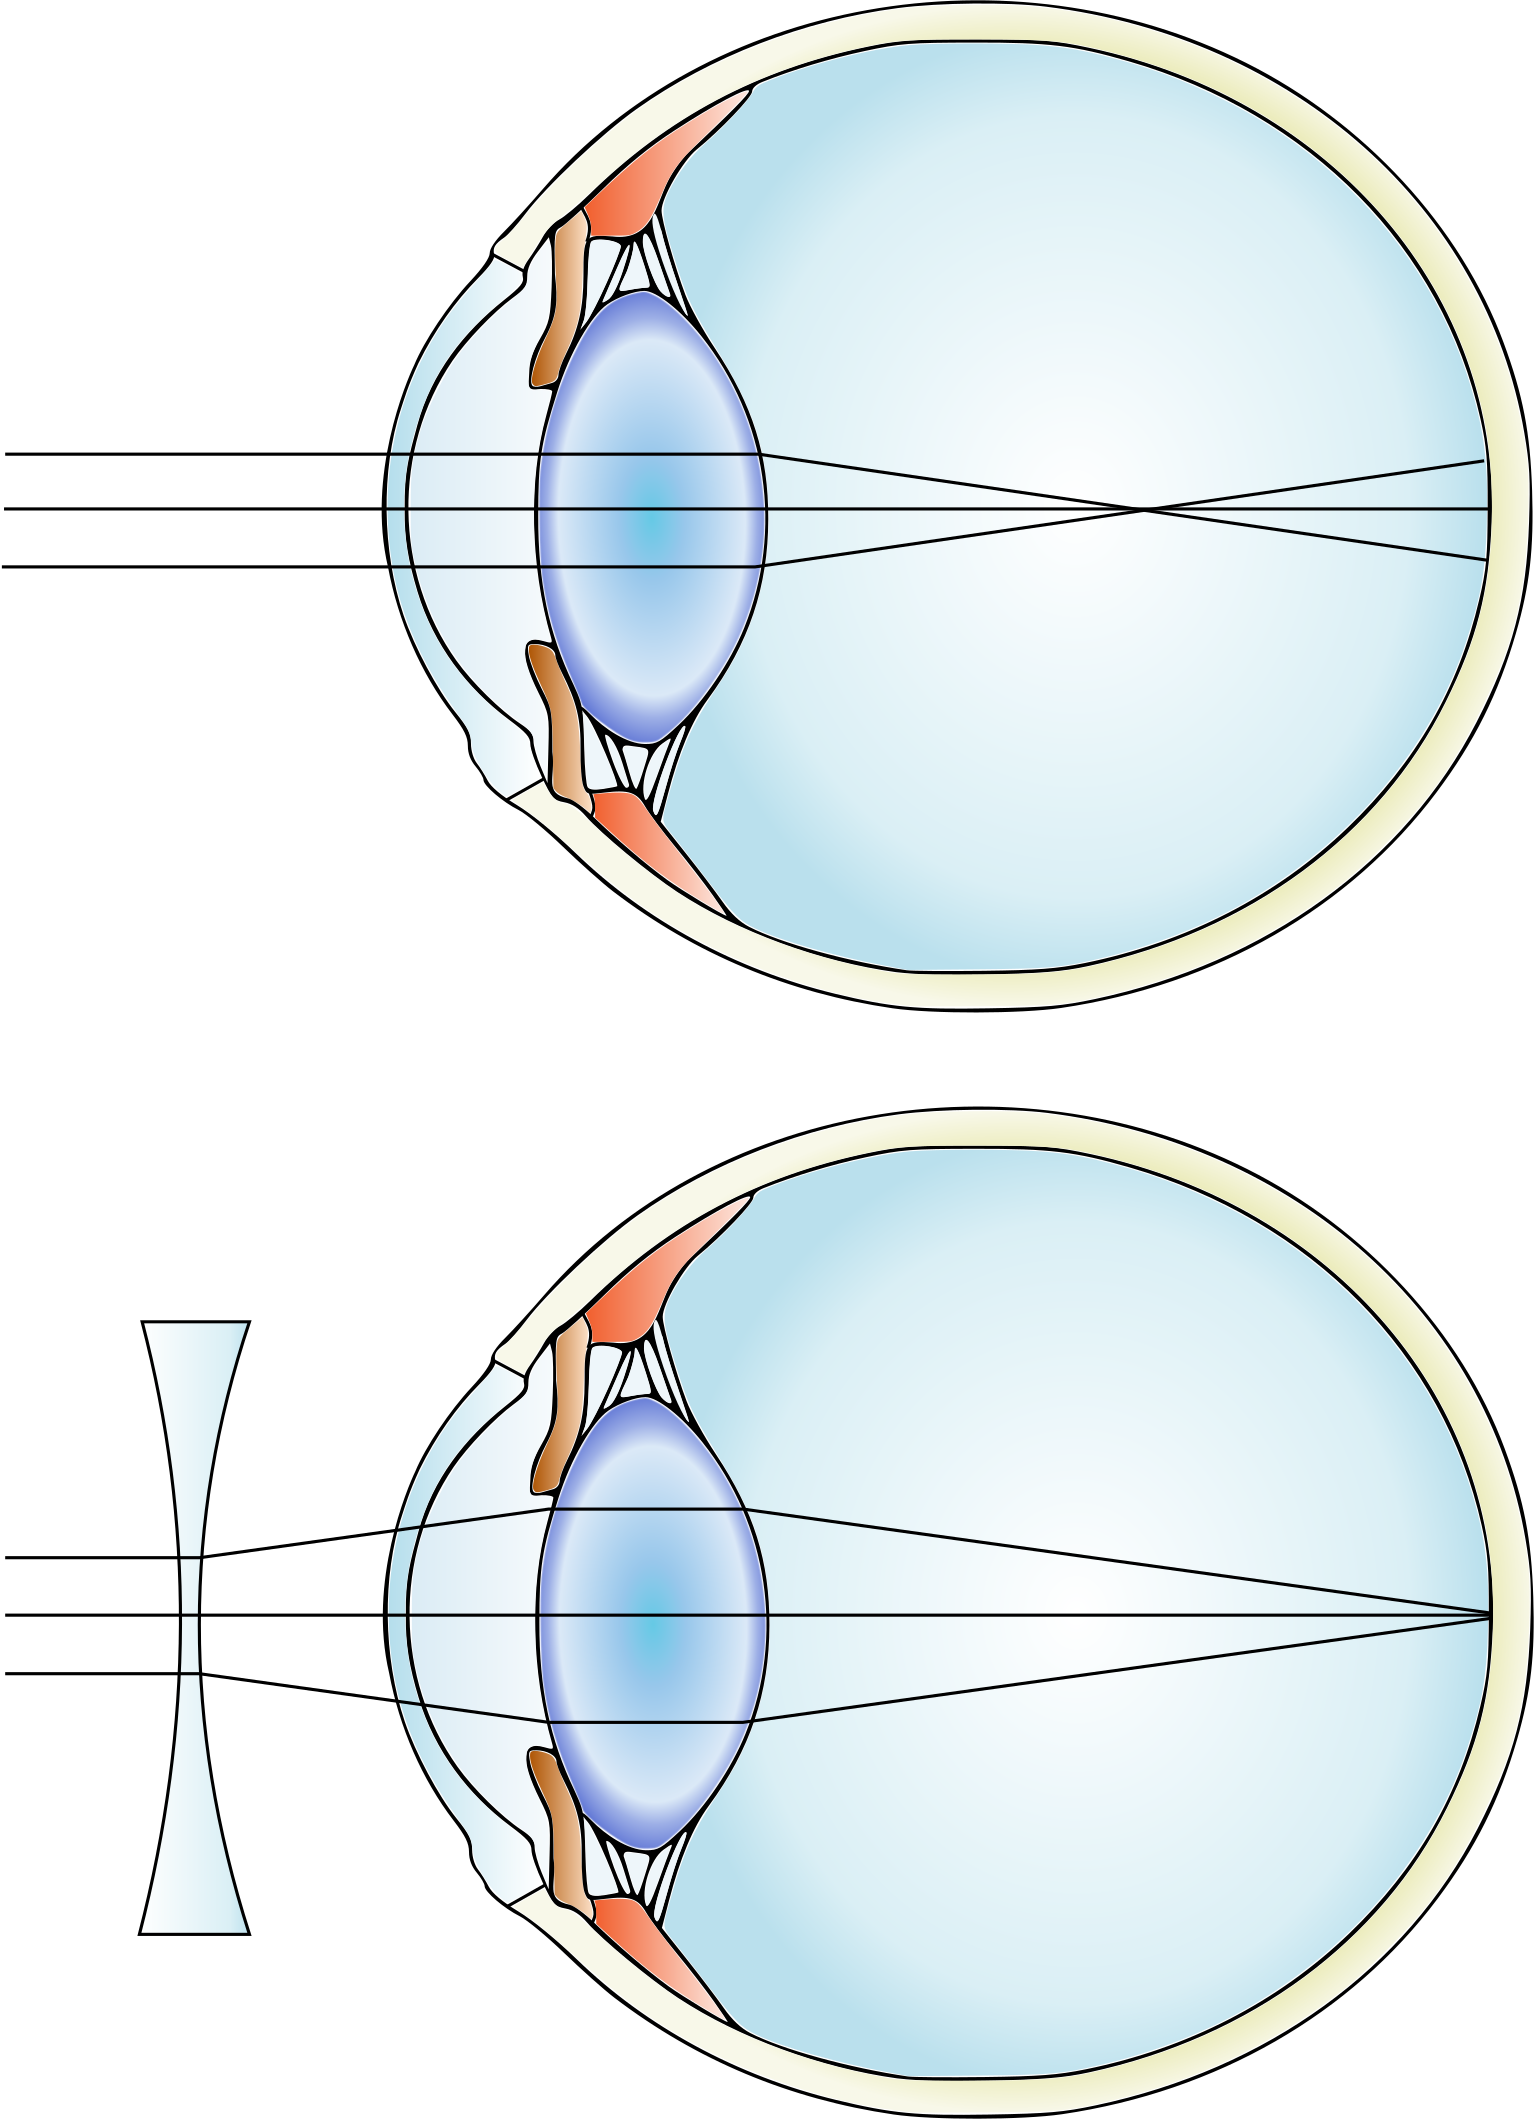
\includegraphics[width=\textwidth]{myopia.png}
\end{center}

\end{column}

\begin{column}{5cm}


\pause

Aber wie gehts weiter?

\end{column}


\end{columns}

    
\end{frame}


 
% %% %% TLIA
\begin{frame}

 \frametitle{In dieser Vorlesung geht es um \dots}

\dots die Sehbahn von den Rezeptoren aufwärts.

\begin{center}
    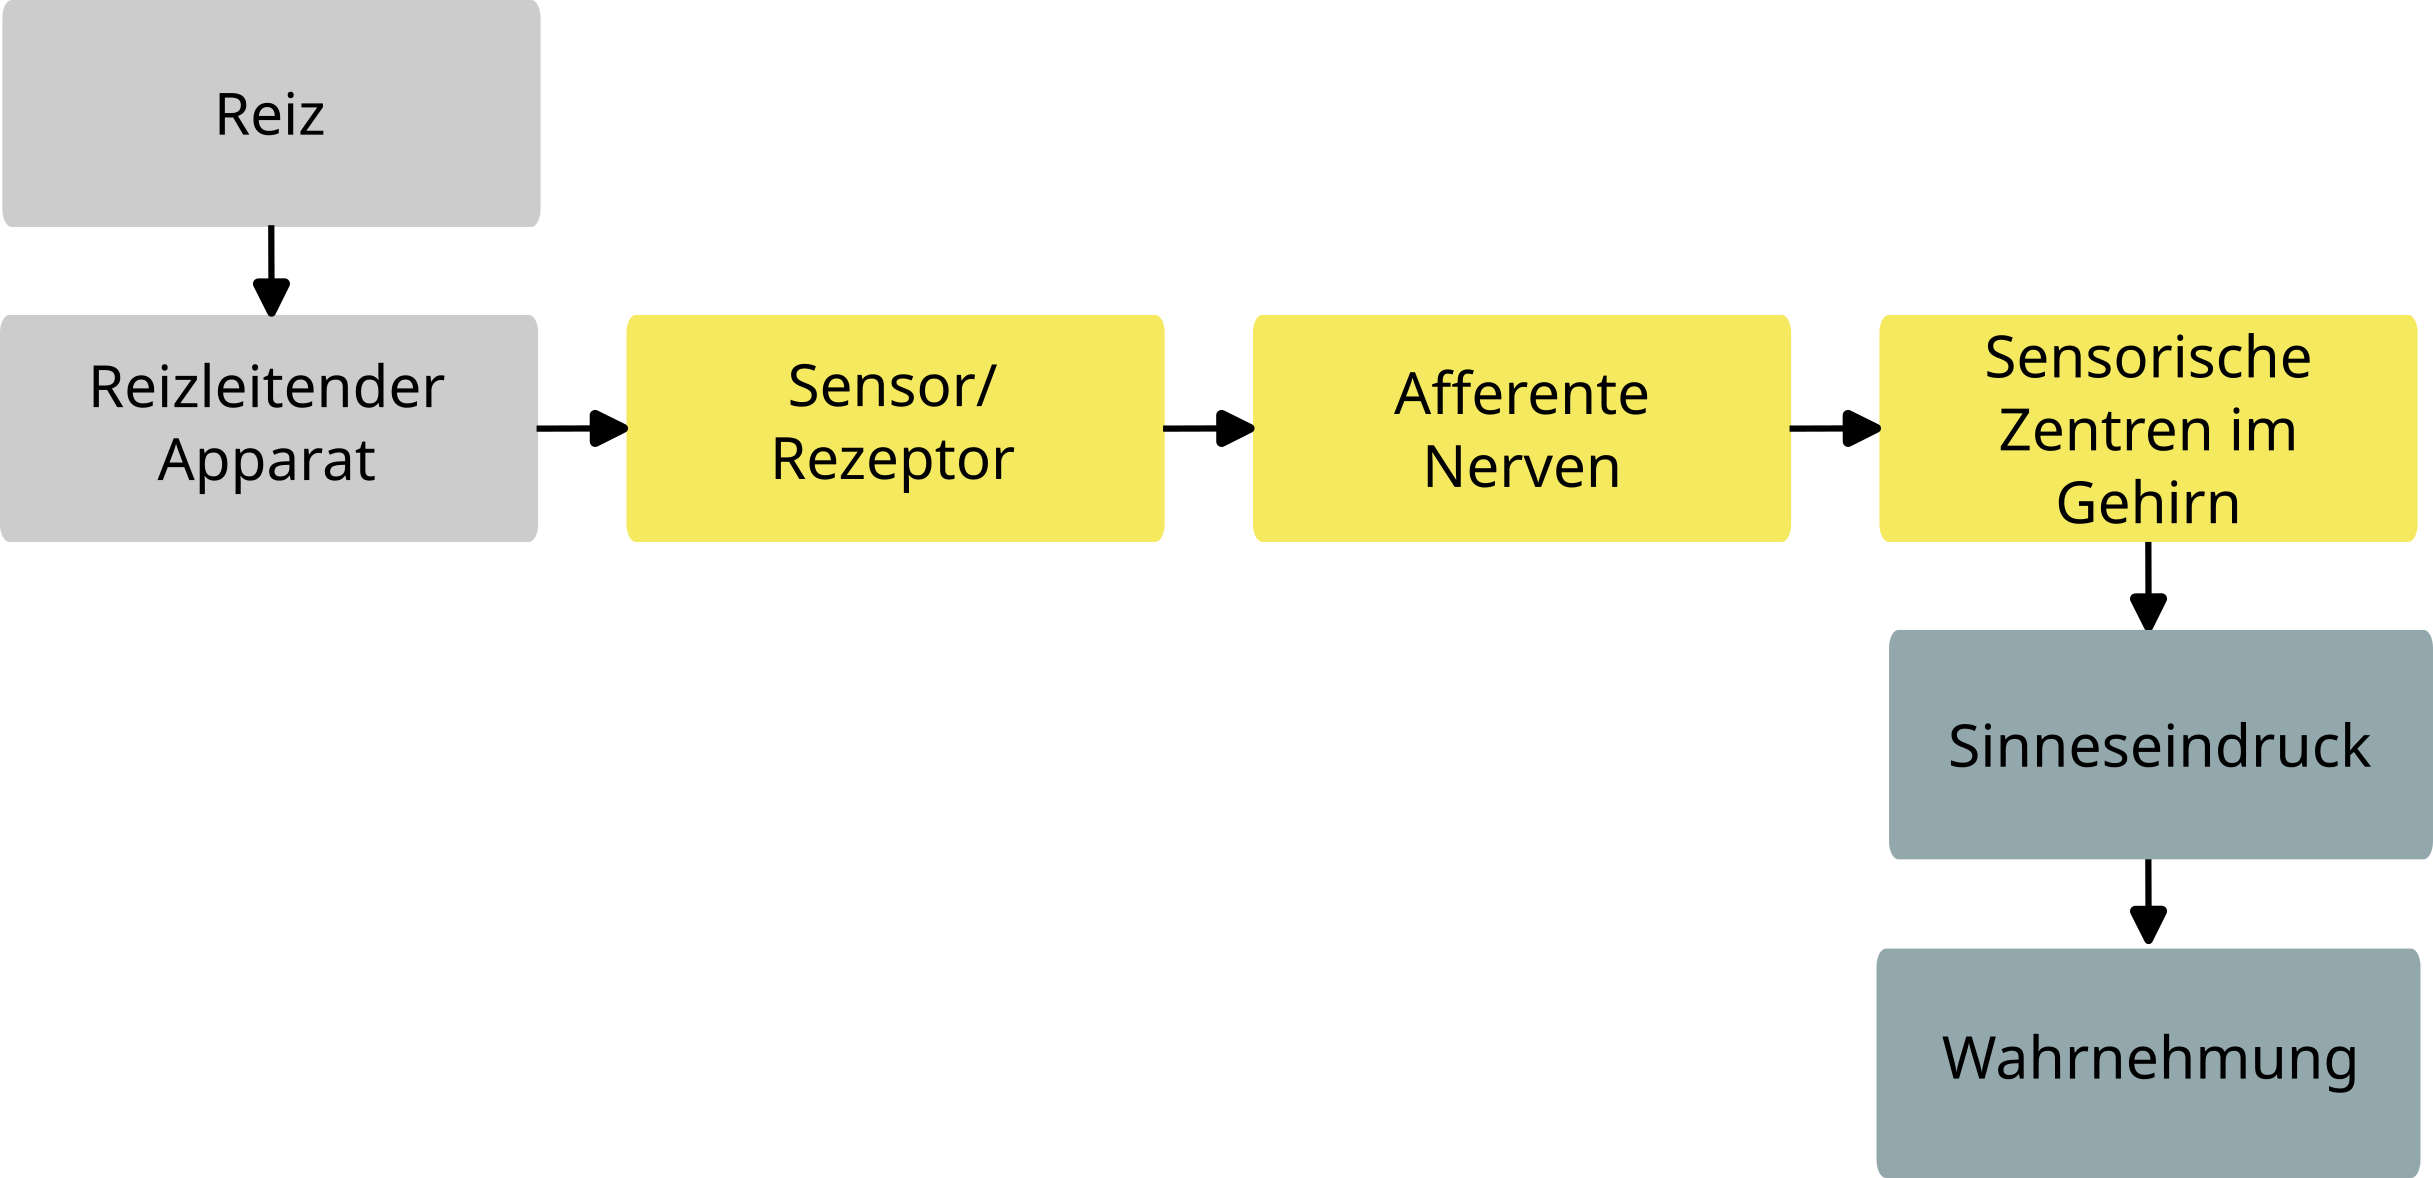
\includegraphics[width=\textwidth]{wahrnehmungsprozess_ohne_beispiel_ab_sensor.png}
\end{center}



\end{frame}


%  % Learning Objectives
 
\begin{frame}

 \frametitle{Nach dieser Vorlesung sollten Sie folgendes können}



\begin{block}{Grundlagen:}




\begin{itemize}

    \item 
den Aufbau der Retina beschreiben
    \item 
die Rolle des Pigmentepithels erläutern
    \item 
die molekulare und zellulären Grundlagen der Photorezeption erläutern
    \item 
photopisches und skotopisches Sehen beschreiben und erklären
    \item 
die Physiologie des Farbsehens beschreiben
    \item 
die Anatomie der Sehbahn beschreiben
    \item 
die Rolle von kortikalen Regionen beim Sehen beschreiben
    \item 
die Rolle efferenter Verbindungen beim Sehen erläutern
    \item 
die Grundlagen des Tiefensehens erklären
\end{itemize}


\end{block}

\end{frame}

\begin{frame}

 \frametitle{Nach dieser Vorlesung sollten Sie folgendes können}

 

\begin{block}{Klinik:}

\begin{itemize}
    
\item 
Anomalien im Farbsehen benennen und erklären
    \item 
Perimetrie beschreiben und Anwendungen erklären
    \item 
Ausfälle des Gesichtsfeldes erklären und beschreiben
    \item 
Diplopie definieren und erklären
    \item 
Strabismus definieren und erklären

\end{itemize}


\end{block}



\end{frame}



%% %% %% Main Body


%%%%%%%%%%%%%%%%%%%%%%%%%%%%%%%%%%%%%%%%%
%% Wahrnehmungsbahn: Sensor/Rezeptor
%%%%%%%%%%%%%%%%%%%%%%%%%%%%%%%%%%%%%%%%%

%% Aufbau der Retina 3-11

%% Phototransduktion 12-23


%% Retinale Signalverarbeitung: Bipoalarzellen 28-49

%% Sehen bei Tag und Nacht: Farbensehen 24-27, Adaptation 50-54


%%%%%%%%%%%%%%%%%%%%%%%%%%%%%%%%%%%%%%%%%
%% Wahrnehmungsbahn: Afferente Nerven
%%%%%%%%%%%%%%%%%%%%%%%%%%%%%%%%%%%%%%%%%

%% Retinale Ganglienzellen (Buch)

%% Verlauf der Sehbahn 58

%% Gesichtsfeld, Skotome, Perimetrie 57, 59





%%%%%%%%%%%%%%%%%%%%%%%%%%%%%%%%%%%%%%%%%
%% Sensorische Zentren Sinneseindruck, Wahrnehmung
%%%%%%%%%%%%%%%%%%%%%%%%%%%%%%%%%%%%%%%%%

%% Gehirnregionen und Funktion

%% Von Form zu Objekt

%% Tiefensehen

%% Efferente Bahnen: Augenbewegungen, Pupille + Diplope  + Strabismus







%% IMPP Frage, Einfügen an geeignetem ort

\begin{frame}{IMPP Frage}

Welche Aussage zur Wellenlänge (in nm) des Absoprtionsmaximums der Stäbchen in der Netzhaut trifft typischerweise zu?

\begin{description}
\item[A.] Sie ist größer als die der Grünzapfen (M-Zapfen)
\item[B.] Sie ist größer als die der Rotzapfen (L-Zapfen) 
\item[C.] Sie ist kleiner als die der Blauzapfen (K-Zapfen) 
\item[D.] Sie liegt zwischen der der Blauzapfen (K-Zapfen) und der der Grünzapfen (M-Zapfen) %% richtig
\item[E.] Sie liegt zwischen der der Grünzapfen (M-Zapfen) und der der Rotzapfen (L-Zapfen) 
\end{description}

    
\end{frame}

%% Auflösung: Bild Cone-response.svg
\begin{frame}{IMPP Frage}
    
    \begin{center}
        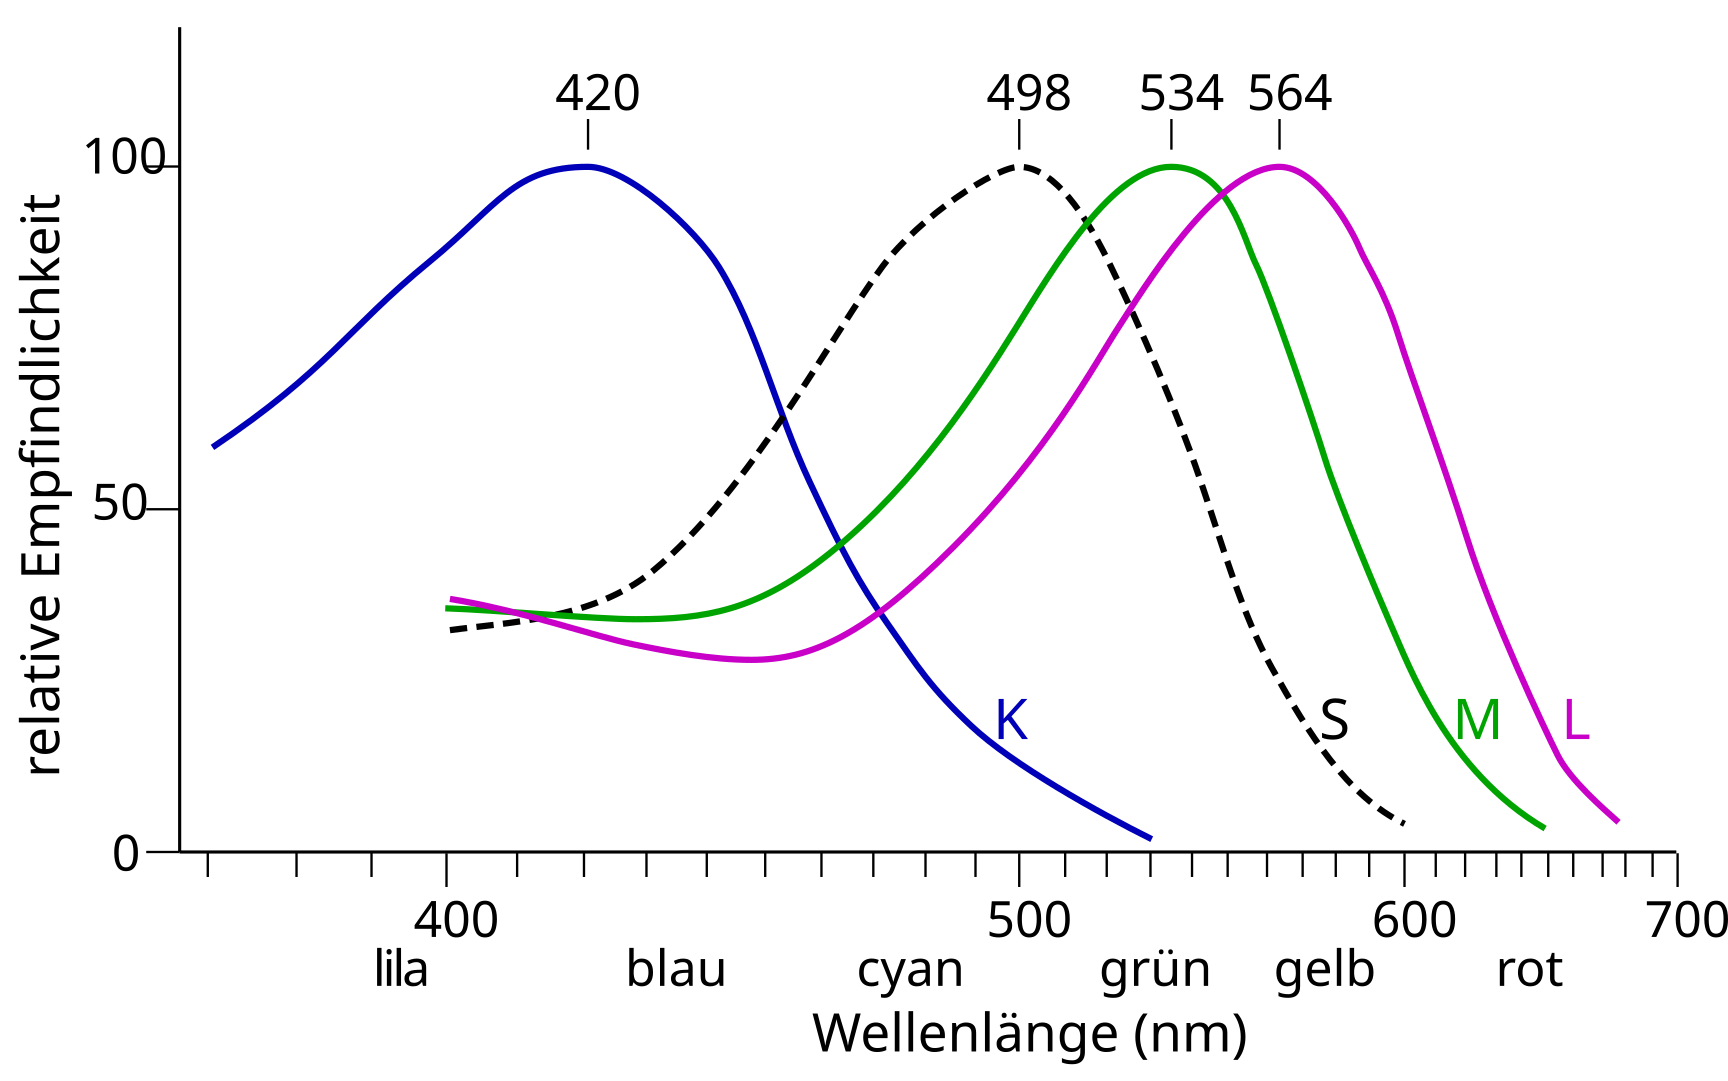
\includegraphics[width=\textwidth]{Cone-response-de.png}
    \end{center}
    
\end{frame}


\begin{frame}{IMPP Frage}

Welche der folgenden Aussagen zu retinalen Ganglienzellen trifft charakteristischerwiese zu?

\begin{description}
\item[A.] Off-Ganglienzellen erhalten Signale direkt von Bipolarzellen, die über ionotrope Glutamatrezeptoren direkt von Zapfen depolarisiert werden. %% richtig
\item[B.] Off-Ganglienzellen erhalten Signale direkt von Bipolarzellen, die über metabotrope Glutamatrezeptoren direkt von Zapfen hyperpolarisiert werden. 
\item[C.] Off-Ganglienzellen erhalten Signale direkt von Zapfen, die bei Belichtung vermehrt GABA freisetzen.
\item[D.] Off-Ganglienzellen erhalten Signale direkt von Zapfen, die bei Belichtung vermehrt Glutamat freisetzen.
\item[E.] Off-Ganglienzellen erhalten Signale direkt von Zapfen, die durch Belichtung depolarisert werden.
\end{description}

    
\end{frame}

%% Auflösung: Bild retina 


\begin{frame}{IMPP Frage}
\begin{center}
    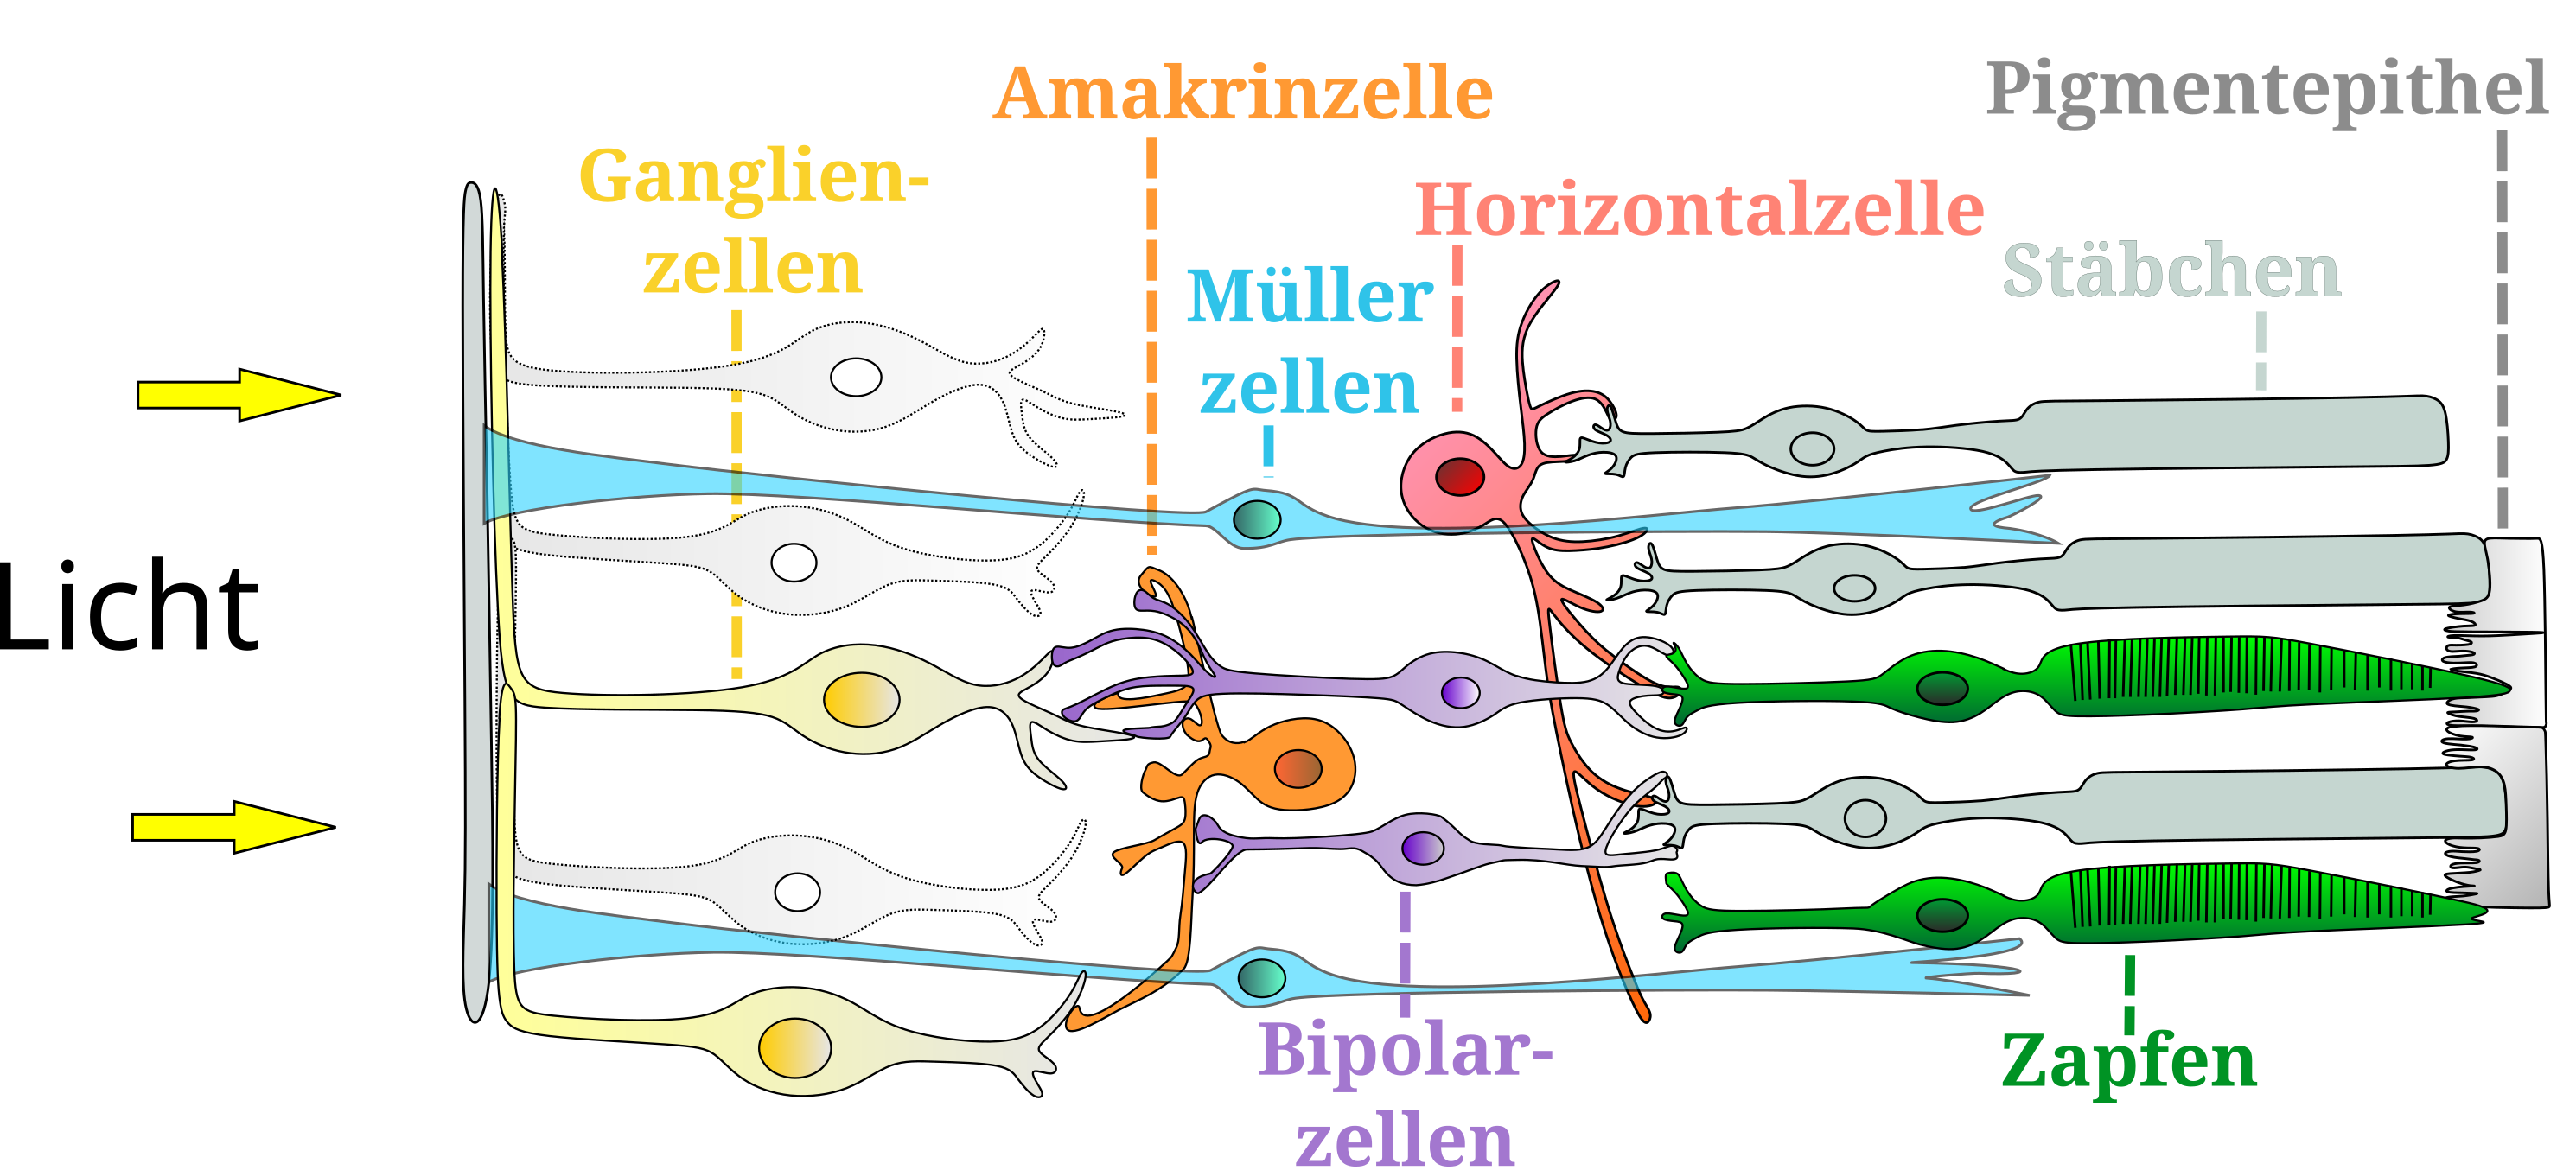
\includegraphics[width=\textwidth]{Retina_de.png}
\end{center}
\end{frame}


%% Auflösung: Bild on/off ganglien
\begin{frame}{IMPP Frage}
\begin{center}
    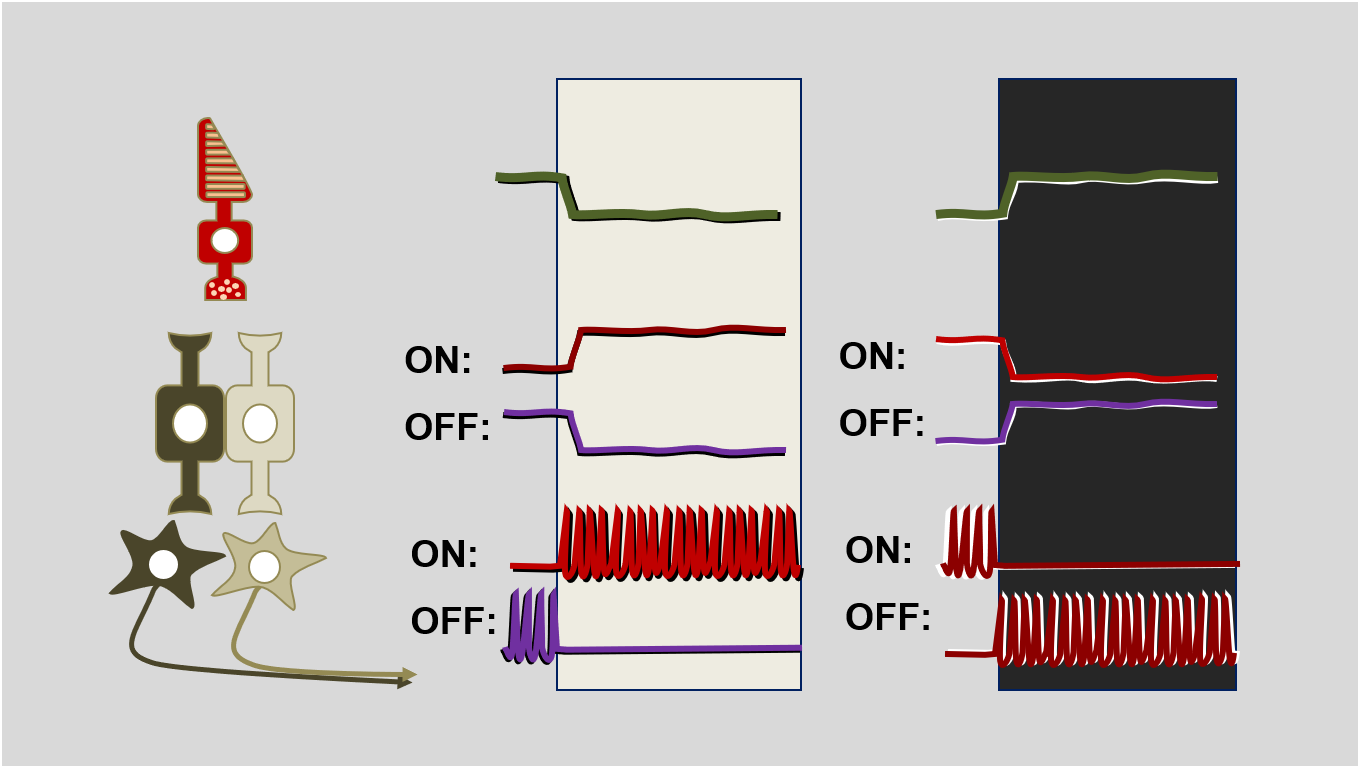
\includegraphics[width=\textwidth]{on_off_bipolarzellen.png}
\end{center}

Off-Ganglienzellen erhalten Signale direkt von Bipolarzellen,
die  ̈uber ionotrope Glutamatrezeptoren direkt von Zapfen
depolarisiert werden.

\end{frame}



%% %% %% %% Review


\begin{frame}

 \frametitle{Jetzt* sollten Sie folgendes können}



\begin{block}{Grundlagen:}




\begin{itemize}

    \item 
den Aufbau der Retina beschreiben
    \item 
die Rolle des Pigmentepithels erläutern
    \item 
die molekulare und zellulären Grundlagen der Photorezeption erläutern
    \item 
photopisches und skotopisches Sehen beschreiben und erklären
    \item 
die Physiologie des Farbsehens beschreiben
    \item 
die Anatomie der Sehbahn beschreiben
    \item 
die Rolle von kortikalen Regionen beim Sehen beschreiben
    \item 
die Rolle efferenter Verbindungen beim Sehen erläutern
    \item 
die Grundlagen des Tiefensehens erklären
\end{itemize}


\end{block}

\end{frame}

\begin{frame}

 \frametitle{Jetzt* sollten Sie folgendes können}

 

\begin{block}{Klinik:}

\begin{itemize}
    
\item 
Anomalien im Farbsehen benennen und erklären
    \item 
Perimetrie beschreiben und Anwendungen erklären
    \item 
Ausfälle des Gesichtsfeldes erklären und beschreiben
    \item 
Diplopie definieren und erklären
    \item 
Strabismus definieren und erklären

\end{itemize}


\end{block}



\end{frame}





%% Feedbackhinweisblock
\begin{frame}
\frametitle{Danke für Ihr Feedback!}

\begin{columns}[c]

\begin{column}{6cm}
\begin{center}
 
\includegraphics[width=\textwidth]{smilie_balloons.jpg}
\end{center}

\end{column}

\begin{column}{4cm}


\begin{center}

\includegraphics[width=\textwidth]{feedback_QR.png}
\end{center}
\end{column}


\end{columns}
\end{frame}




%% %% %% Bildnachweis


\begin{frame}
\frametitle{Bildnachweis}
\begin{tiny}



 
\begin{itemize}


\item
Absorptionskurven für Stäbchen- und Zapfenzellen. Modifiziert von mir (Farbe geändert, um für Farebenblinde besser lesbar zu sein; Buchstaben-Bezeichnungen modifiziert). Vorlage von Cone-response.svg: w:User:DrBob and w:User:Zeimusuderivative work: Sgbeer - Cone-response.svg (Vectorized version of the GFDL image Cone-response.png uploaded by User:Maxim Razin based on work by w:User:DrBob and w:User:Zeimusu.), CC BY-SA 3.0, \url{https://commons.wikimedia.org/w/index.php?curid=17729332}

\item
Aktivierungsmuster von On- und Off-Bipolarzellen und On- und Off-Ganglienzellen. Cristiane Tilelli, CC BY-SA 4.0 \url{https://creativecommons.org/licenses/by-sa/4.0}, via Wikimedia Commons
  
\item
Korrektur von Kurzsichtigkeit mithilfe einer Streulinse. By Gumenyuk I.S. - Own work, CC BY-SA 4.0, \url{https://commons.wikimedia.org/w/index.php?curid=46820576}

\item
Luftballons mit frohen und traurigen Smileys. Photo by \href{https://unsplash.com/@artbyhybrid?utm_source=unsplash&utm_medium=referral&utm_content=creditCopyText}{Hybrid} on \href{https://unsplash.com/s/photos/feedback?utm_source=unsplash&utm_medium=referral&utm_content=creditCopyText}{Unsplash}

\item
Wahrnehmungsbahn und einzelne Prozesse entlang der Wahrnehmungsbahn (mehrere Bilder). Mein eigenes Werk, CC BY-SA 4.0, 2022. 

\item
Zellen der Retina. Modifiziert von mir, CC BY-SA 4.0, 2022, nach einer Vorlage von  Pancrat, CC BY-SA 4.0 \url{https://creativecommons.org/licenses/by-sa/4.0}, via Wikimedia Commons

\end{itemize}
\end{tiny}
\end{frame}






\end{document}

%%% Frequently used snippets

%% \begin{columns}[c]

%% \begin{column}{5cm}
%% \end{column}

%% \begin{column}{5cm}
%% \end{column}


%% \end{columns}




